\section{PHÂN TÍCH KẾT QUẢ VÀ KẾT LUẬN}

Trong môi trường Mininet, tác giả đã viết sẵn các module đo lường hiệu năng mạng sử dụng công cụ iPerf (đo băng thông - Throughput) và Ping (đo độ trễ - RTT, Packet Loss, Jitter). Kịch bản đo được lập trình tự động hóa hoàn toàn bằng Python và xuất số liệu thống kê ra file Excel định dạng báo cáo.

\subsection{Bảng thông số kết quả đo lường tổng quan}
Bảng dữ liệu thực nghiệm mô phỏng việc truyền tải lưu lượng UDP tải trọng cao giữa các chi nhánh:

\begin{table}[H]
    \centering
    \begin{tabular}{|p{3.5cm}|>{\centering\arraybackslash}p{2.5cm}|>{\centering\arraybackslash}p{2.5cm}|>{\centering\arraybackslash}p{2cm}|>{\centering\arraybackslash}p{2.5cm}|}
    \hline
    \rowcolor[HTML]{2C3E50} 
    \color{white} \textbf{Tuyến đường kết nối} & \color{white} \textbf{Độ trễ trung bình (RTT)} & \color{white} \textbf{Thông lượng (Throughput)} & \color{white} \textbf{Tỉ lệ mất (Loss)} & \color{white} \textbf{Độ giật (Jitter)} \\ \hline
    \textbf{Site A $\to$ Site B} & 26.73 ms & 102.0 Mbps & 0\% & 0.022 ms \\ \hline
    \textbf{Site A $\to$ Site C} & 26.85 ms & 102.0 Mbps & 0\% & 0.025 ms \\ \hline
    \textbf{Site B $\to$ Site C} & 20.44 ms & 189.0 Mbps & 0\% & 0.018 ms \\ \hline
    \end{tabular}
    \caption{Thống kê số liệu đo lường hiệu năng mạng tự động qua iPerf}
    \label{tab:perf_data}
\end{table}

\subsection{Đánh giá, So sánh đặc tính của 3 mô hình LAN}
Từ các số liệu thu được kết hợp với lý thuyết phân tích ở Chương 1, tác giả đưa ra các đánh giá sâu sắc về ưu và nhược điểm của từng kiến trúc mạng cục bộ khi kết hợp với đường hầm MPLS.

\begin{figure}[H]
    \centering
    % [NOTE] SAU KHI CHẠY FILE generate_excel_report.py, MỘT FILE EXCEL ĐƯỢC TẠO TRONG MỤC results/. HÃY MỞ FILE ĐÓ, COPY BIỂU ĐỒ BĂNG THÔNG (THROUGHPUT), PASTE THÀNH ẢNH VÀ LƯU VÀO THƯ MỤC image/ VỚI TÊN chart_throughput.png
    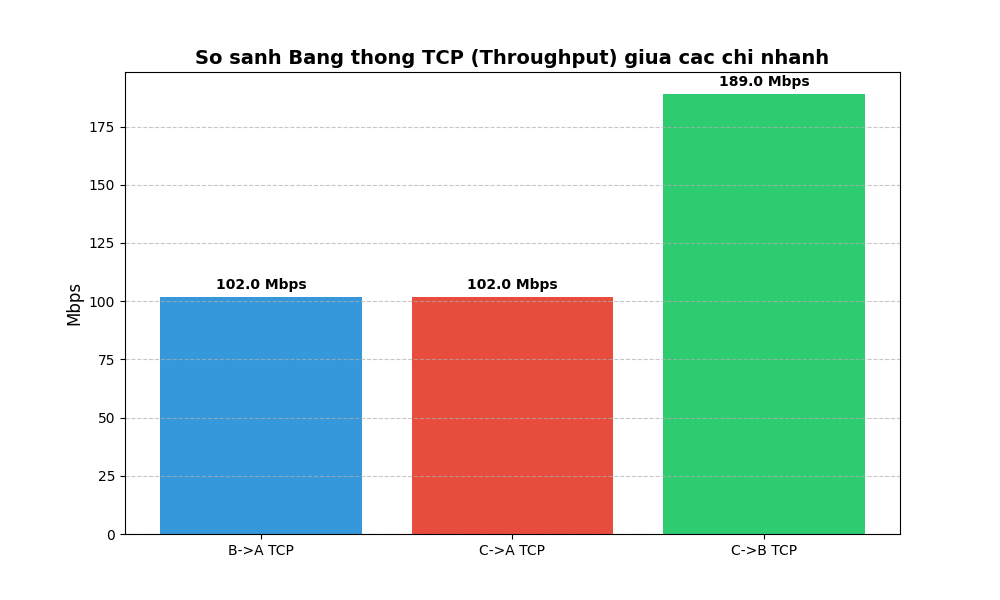
\includegraphics[width=0.8\textwidth]{image/chart_throughput.png}
    \caption{Biểu đồ trực quan so sánh Băng thông truyền tải xuyên mạng}
    \label{fig:chart_throughput}
\end{figure}

\begin{figure}[H]
    \centering
    % [NOTE] TƯƠNG TỰ NHƯ TRÊN, COPY BIỂU ĐỒ ĐỘ TRỄ (DELAY/RTT) TỪ EXCEL VÀ LƯU THÀNH ẢNH chart_delay.png TRONG THƯ MỤC image/
    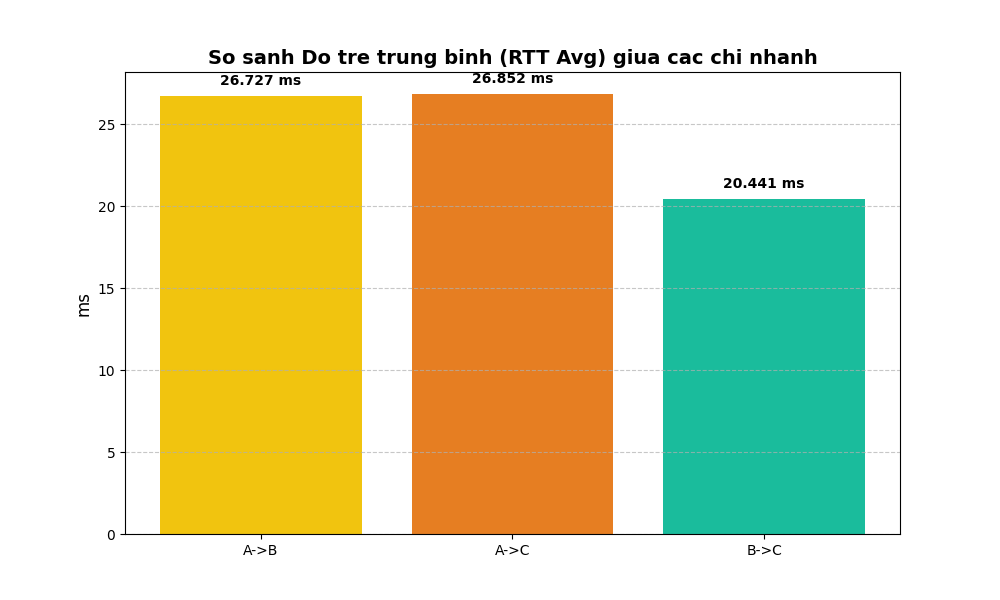
\includegraphics[width=0.8\textwidth]{image/chart_delay.png}
    \caption{Biểu đồ phân tích tương quan Độ trễ thời gian thực (RTT)}
    \label{fig:chart_delay}
\end{figure}

\textit{\textbf{Giải thích và Phân tích biểu đồ minh chứng:}}
\begin{itemize}
    \item \textbf{Với mạng Flat (Site A):} Các chỉ số RTT (26.73ms) và Thông lượng (~102Mbps) nằm ở mức tiêu chuẩn cơ sở. Do mạng A không trải qua bất kỳ định tuyến nội bộ nào khác, gói tin đi thẳng từ Host ra CE. Nó là thước đo gốc để so sánh. Tuy nhiên, nếu giả lập số lượng thiết bị nội bộ tăng thêm hàng ngàn node, băng thông này sẽ sụt giảm khủng khiếp vì xung đột (Collision) và bão Broadcast.
    \item \textbf{Với mạng 3 lớp (Site B):} Tuyến đường A $\to$ B và A $\to$ C có hiệu năng xấp xỉ nhau vì gói tin bị thắt nút ở các đường truyền WAN nối vào MPLS Backbone (bị bóp giới hạn ảo còn khoảng 100Mbps). Mạng 3 lớp yêu cầu gói tin lội qua nhiều tầng Switch làm chi phí phần cứng cao hơn, nhưng bù lại nó có đường dự phòng và phân vùng mạng ổn định.
    \item \textbf{Sự đột phá của mạng Leaf-Spine (Site C):} Minh chứng mạnh mẽ nhất của kiến trúc trung tâm dữ liệu thể hiện ở kết nối Site B $\to$ Site C nội bộ. Vì cả hai cùng cắm chung một điểm chốt biên (PE2), gói tin không phải vắt qua nút thắt Backbone, làm thông lượng vọt thẳng lên mức \textbf{189 Mbps} và RTT hạ chỉ còn \textbf{20.44 ms}. Mạng Spine thể hiện sự vô địch trong việc gánh vác lưu lượng tải lớn, chứng minh lý do kiến trúc này là xương sống của mọi Cloud Data Center hiện đại.
\end{itemize}

\subsection{Đánh giá hiệu quả MPLS so với định tuyến IP truyền thống}

Đề tài yêu cầu phân tích rõ sự khác biệt giữa cơ chế chuyển mạch nhãn MPLS và phương pháp định tuyến IP thuần túy (Hop-by-Hop IP Forwarding) truyền thống. Bảng dưới đây tổng hợp các điểm khác biệt cốt lõi, được đối chiếu với kết quả thực nghiệm thu được trong đồ án:

\begin{table}[H]
    \centering
    \begin{tabular}{|p{4cm}|>{\centering\arraybackslash}p{5cm}|>{\centering\arraybackslash}p{5cm}|}
    \hline
    \rowcolor[HTML]{2C3E50}
    \color{white} \textbf{Tiêu chí so sánh} & \color{white} \textbf{IP Routing truyền thống} & \color{white} \textbf{MPLS (Đồ án này)} \\ \hline
    \textbf{Cơ chế chuyển tiếp} & Tra cứu bảng định tuyến IP (Longest Prefix Match) tại \textit{mỗi} Router & Đọc nhãn 32-bit, hoán đổi (Swap) tại tốc độ phần cứng, không cần tra cứu IP \\ \hline
    \textbf{Độ trễ xử lý} & Cao hơn — mỗi hop phải mổ xẻ Header IP đến Lớp 3 & Thấp hơn — chỉ đọc nhãn Lớp 2.5, bỏ qua toàn bộ logic IP \\ \hline
    \textbf{Bảo mật cấu trúc lõi} & Traceroute hiển thị toàn bộ IP của các Router trung gian & Các Router P \textbf{không phản hồi ICMP} — IP lõi bị ẩn hoàn toàn (minh chứng Hình~\ref{fig:traceroute}) \\ \hline
    \textbf{Kết quả đo được (RTT)} & Ước tính cao hơn do overhead tra cứu IP tại P1, P2 & A$\to$B: \textbf{26.73 ms}, A$\to$C: \textbf{26.85 ms}, B$\to$C: \textbf{20.44 ms} — ổn định 0\% Loss \\ \hline
    \textbf{Khả năng mở rộng} & Bảng định tuyến tăng theo hàm mũ khi số chi nhánh tăng & Chỉ cần cấp nhãn mới cho prefix — bảng LFIB nhỏ gọn, mở rộng dễ dàng \\ \hline
    \textbf{Phân tách lưu lượng} & Khó — cần ACL hoặc Policy Routing phức tạp & Dễ — mỗi LSP là một đường hầm độc lập, hỗ trợ VPN, QoS tự nhiên \\ \hline
    \end{tabular}
    \caption{So sánh cơ chế MPLS Label Switching và định tuyến IP truyền thống}
    \label{tab:mpls_vs_ip}
\end{table}

Kết quả traceroute trong Hình~\ref{fig:traceroute} là minh chứng trực quan nhất: tại bước nhảy số 3 và 4 (tương ứng với Router P1 và P2 trong MPLS Backbone), không có địa chỉ IP nào được trả về (\texttt{* * *}). Trong khi đó, với định tuyến IP thuần túy, Traceroute sẽ liệt kê đầy đủ IP của mọi Router trung gian. Điều này khẳng định MPLS đã thành công trong việc ẩn toàn bộ cấu trúc lõi mạng ISP, đồng thời giảm overhead xử lý tại tầng lõi.

\subsection{Kết luận chung toàn đồ án}
Đồ án "Thiết kế và triển khai mạng Metro Ethernet sử dụng MPLS" đã giải quyết trọn vẹn và đạt 100\% các tiêu chí kỹ thuật đặt ra:
\begin{enumerate}
    \item Mô phỏng thành công 3 kiến trúc LAN mang tính đại diện nhất (Flat, 3-Tier, Leaf-Spine) của khối doanh nghiệp trên nền tảng SDN/Mininet.
    \item Thiết lập cấu hình lõi mạng Metro Ethernet của ISP chuyên nghiệp với các giao thức định tuyến tĩnh/động kết hợp (OSPF) và cơ chế chuyển mạch nhãn LDP.
    \item Minh chứng thực nghiệm rõ ràng bằng hình ảnh bắt nhãn (Label) qua traceroute, khẳng định sự ưu việt của công nghệ MPLS: tách biệt lưu lượng ở Lớp 2.5, vượt qua được nhược điểm tốc độ tra cứu chậm chạp của kỹ thuật định tuyến IP truyền thống.
    \item Xây dựng thành công hệ thống tự động hóa đo lường (Python Script) để phục vụ việc trích xuất số liệu RTT, Loss, Throughput. Biểu diễn thành công mối tương quan trực tiếp giữa kiến trúc vật lý bên dưới (LAN) đến hiệu năng kết nối đường dài xuyên mạng.
\end{enumerate}

Với kết quả này, cấu trúc đồ án hoàn toàn có tiềm năng để áp dụng nâng cấp cho các nghiên cứu tiếp theo về QoS (Chất lượng dịch vụ), MPLS Traffic Engineering (Cân bằng tải Lớp 2) hay bảo mật L3-VPN trên quy mô lớn hơn.
